\documentclass{zc-ust-hw}

% Shared by every phase report: packages, title block, team, repository link.
\usepackage{booktabs}
\usepackage{microtype}
\hypersetup{colorlinks=true, linkcolor=black, citecolor=black, urlcolor=blue!60!black}
\lstset{language=C++, numbers=none, basicstyle=\ttfamily\footnotesize}
\setlist{itemsep=2pt, topsep=4pt}

% Title block: name / ID / date in a wrapping column beside the logo, so long name or ID
% lists continue on the next line instead of running under the logo.
\makeatletter
\renewcommand{\maketitle}{%
  \noindent
  \begin{minipage}[t]{0.76\linewidth}
    \vspace{0pt}
    \begin{tabular}[t]{@{}l p{0.82\linewidth}@{}}
      \ifx\@name\empty\else Name: & \raggedright \@name \tabularnewline \fi
      \ifx\@id\empty\else ID: & \raggedright \@id \tabularnewline \fi
      Date: & \today
    \end{tabular}
  \end{minipage}\hfill
  \begin{minipage}[t]{0.2\linewidth}
    \vspace{0pt}\raggedleft
    
\includegraphics[height=2cm]{logo.jpg}
  \end{minipage}

  \begin{center}
    \textbf{\large \@course}\\
    \@assignment
  \end{center}

  \noindent\rule{\linewidth}{0.1mm}
  \medskip
}
\makeatother

\newcommand{\repo}{\url{https://github.com/AliAshraf69420/Parallel-Distributed-Project}}

\name{Ali Ashraf Hassan Abdelghany, Ahmad Muhammadi, Omar Ali, Abdullah Ayman}
\id{202301812, 202301826, 202300942, 202301731}
\course{SW 401}

\assignment{Final Report: A Parallel and Distributed Image-Normalization Pipeline}

\begin{document}

\maketitle

\noindent\textbf{Repository:} \repo\\
Its \texttt{README.md} gives the commands that reproduce every number in this report.\\
\textbf{Machine:} AMD Ryzen 7 5800H (8 cores / 16 threads), 14\,GiB RAM, NVMe SSD, RTX 3050 Ti,
Arch Linux, GCC 16.2, OpenMPI 5.0.11, Hadoop 3.4.1, CUDA 13.4. The MPI and Hadoop clusters are
Docker containers on this machine.

%======================================================================
\section{Dataset, preprocessing and the computation}
%======================================================================

\paragraph{Dataset.} CUB-200-2011 (Caltech-UCSD Birds): 11{,}788 JPEG photographs of 200
species, with a train/test split and a bounding box per image. Preprocessing (Python, pinned
conda environment) decodes every image, drops one byte-identical duplicate, converts 8 grayscale
images to RGB, clamps 30 boxes to their image, and then \emph{predecodes} each image once into
raw RGB in 1\,GiB shards with a 32-byte index record per image. Result: 11{,}787 images
(5{,}993 train / 5{,}794 test), \textbf{1.07\,GiB of JPEG becomes 5.90\,GiB of raw pixels}.
Class-stratified, nested subsets of 100\,MB and 500\,MB (and $p\times700$\,MiB for weak scaling)
are cut from it, and for Hadoop every set is also exported as text, one image per line with its
pixels in base64 (8.06\,GiB for the full set, 1.33 times the binary).

\paragraph{Computation.} The input preparation of an image classifier: (1) crop each image to
its bounding box and resize it to $224\times224$ (bilinear); (2) \emph{pass 1}: mean and standard
deviation of each colour channel over the training images; (3) \emph{pass 2}: normalize every
image, $x'=(x/255-\mu_c)/\sigma_c$, into a float32 tensor. Pass 1 is a global reduction and pass
2 needs its result, so every parallel model must supply a merge and a synchronization point
between the passes.

\paragraph{Exact by construction.} The computation is specified with integers (fixed-point
resize; exact sums $n$, $\sum v$, $\sum v^2$; a lookup table for normalization), so merging
partial results is integer addition, independent of order. A NumPy reference fixes the expected
statistics and two CRC-32 values per image. \textbf{Every implementation must match it bit for
bit}, and all six do, on all three sets (Table~\ref{tab:models}).

\begin{table}[H]
\centering\small\setlength{\tabcolsep}{5pt}
\begin{tabular}{llll}
\toprule
Version & Model & Merge of pass 1 & Barrier between passes \\
\midrule
Sequential C++ & baseline & -- & -- \\
OpenMP & shared memory & user-defined \texttt{reduction} & end of parallel region \\
C++ threads & shared memory & per-worker sums & \texttt{join} \\
MPI (+ hybrid) & distributed memory & \texttt{MPI\_Allreduce} & the \texttt{Allreduce} \\
Hadoop Streaming & MapReduce & combiner + reducer & job boundary \\
CUDA (bonus) & GPU & block reduction per image & host \\
\bottomrule
\end{tabular}
\caption{The six implementations. All share one C++ library (\texttt{src/common}) for the
kernels, so only the parallel structure differs.}
\label{tab:models}
\end{table}

%======================================================================
\section{Phase 1: shared memory}
%======================================================================

Both passes are an OpenMP \texttt{parallel for} over images, with a user-defined reduction for
the seven counters of pass 1 and no locks anywhere. A second version uses \texttt{std::thread}
with bounded queues (reader $\to$ workers $\to$ writer). On the full set the sequential baseline
needs 9.79\,s of compute; \textbf{OpenMP reaches 7.23$\times$ on 8 cores} (efficiency 0.90,
serial fraction $f\approx0.015$) and the thread pipeline 7.30$\times$
(Figure~\ref{fig:scaling}a). Weak scaling gives a scaled speedup of 7.02 at 8 threads. Three
findings from the profiling:
\begin{itemize}
  \item \textbf{The missing 10\,\% is clock frequency, not serial code.} \texttt{perf} shows
    identical instruction counts at 1 and 8 threads, while the effective clock falls from 3.93
    to 3.55\,GHz ($3.55/3.93=0.90$).
  \item \textbf{Scheduling does not matter here.} We expected \texttt{dynamic} to win because
    crop sizes vary 24 times, but the resize cost depends on the fixed output size: per-image
    time has a coefficient of variation of 0.03, and all schedules are within 4\,\%.
  \item \textbf{Memory hierarchy.} Load latency steps at exactly the cache sizes (1.2\,ns L1,
    3.3\,ns L2, 11\,ns L3, 65--122\,ns DRAM). A column-major resize causes 27 times more cache
    misses for identical output. Per-thread counters packed into shared cache lines are 17.9
    times slower than register-local ones (false sharing).
\end{itemize}

\begin{figure}[H]
\centering
\begin{subfigure}{0.49\linewidth}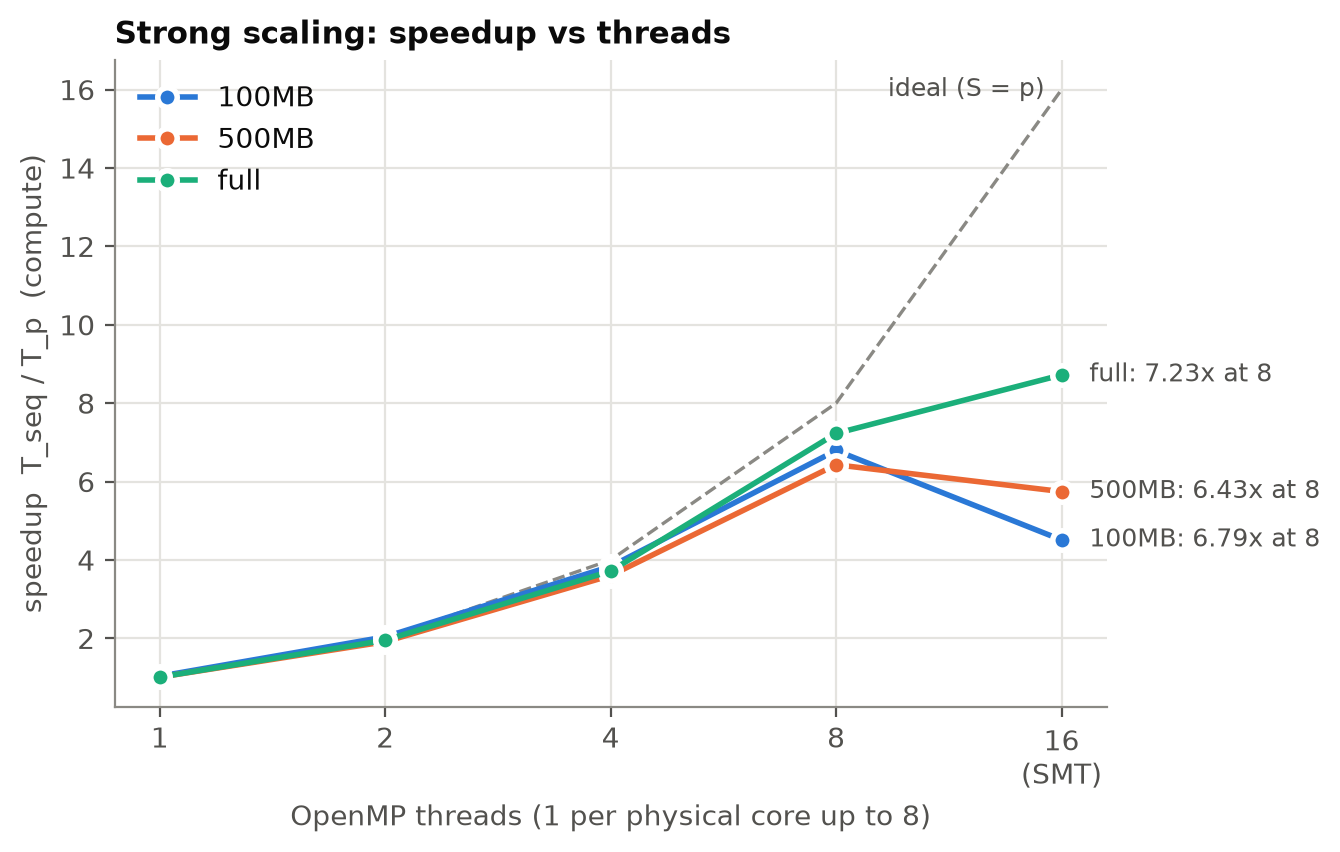
\includegraphics[width=\linewidth]{../plots/phase1/speedup.png}\caption{}\end{subfigure}\hfill
\begin{subfigure}{0.49\linewidth}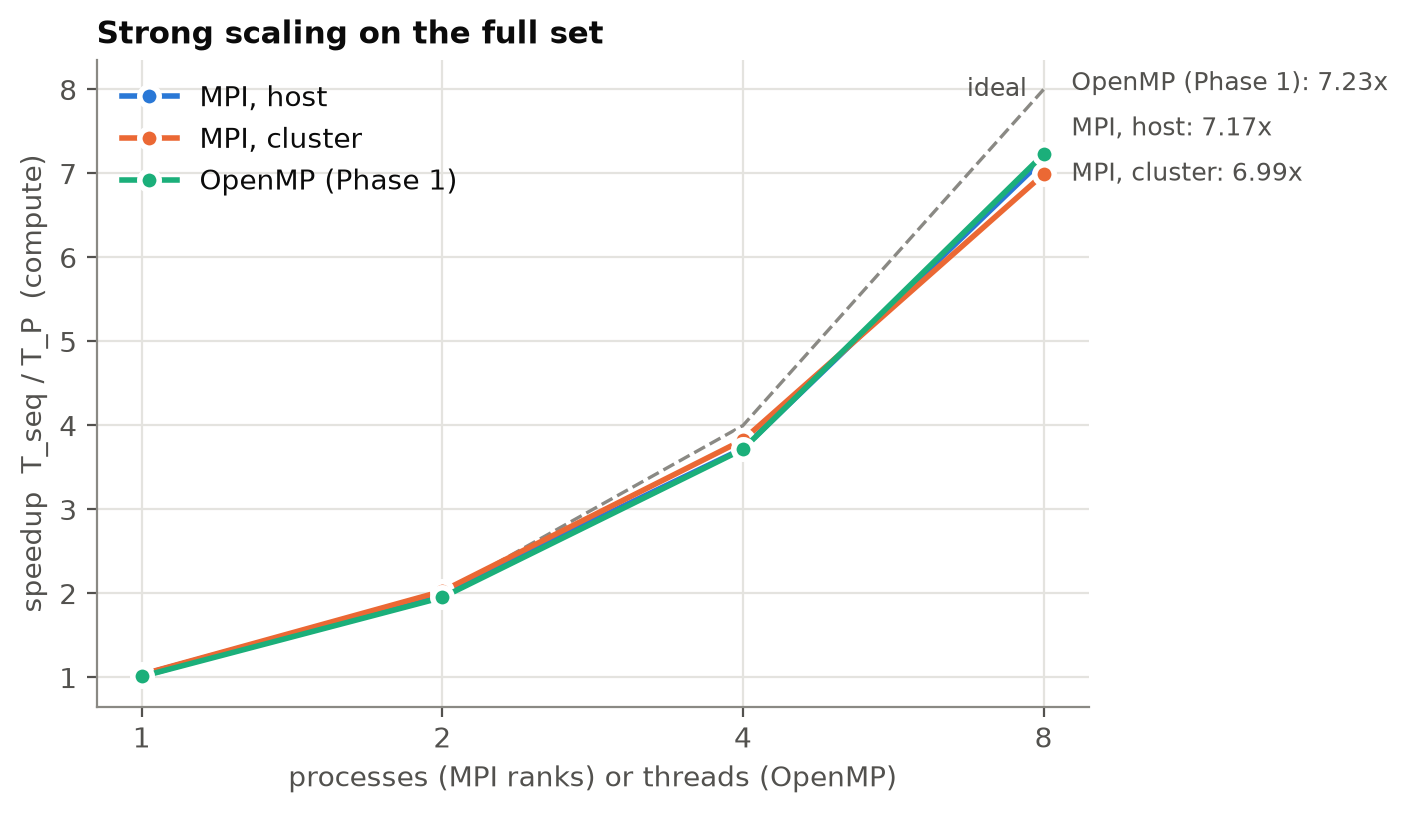
\includegraphics[width=\linewidth]{../plots/phase2/strong.png}\caption{}\end{subfigure}
\caption{Strong scaling. (a) OpenMP, three input sizes. (b) MPI on one host and on the 4-node
container cluster, against OpenMP, full set.}
\label{fig:scaling}
\end{figure}

%======================================================================
\section{Phase 2: distributed memory (MPI)}
%======================================================================

\paragraph{Decomposition.} A block partition of the records. Rank 0 alone reads the index and
sends each rank its block of records (\texttt{MPI\_Send}); every rank then reads its own pixels.
Pass 1 ends in one \texttt{MPI\_Allreduce} over seven integers, and the CRCs and timings return
with \texttt{MPI\_Gatherv} and \texttt{MPI\_Gather}. The application exchanges about 0.4\,MiB to
process 5.9\,GiB, so communication is under 0.1\,\% of the run time.

\paragraph{Results.} At 8 processes MPI reaches \textbf{7.17$\times$} on one host and
6.99$\times$ on four containers connected by TCP (Figure~\ref{fig:scaling}b), with weak-scaling
speedups of 6.98 and 6.91. End to end MPI beats OpenMP (7.14$\times$ against 6.27$\times$),
because each rank opens only its own part of the data. Ping-pong shows a latency-bound region
(12.5\,\textmu s round trip up to 1\,KiB across containers, 0.5\,\textmu s in shared memory) and
a bandwidth-bound one above 64\,KiB. When workers ship every 588\,KiB tensor to rank 0,
\texttt{MPI\_Isend} overlapped with computation hides 95--99\,\% of the send time with one
worker, and nothing once three or more workers saturate the single collector.

%======================================================================
\section{Phase 3: MapReduce on Hadoop}
%======================================================================

\paragraph{Pipeline.} Two Hadoop Streaming jobs with C++ programs (\texttt{src/hadoop/}):
\begin{itemize}
  \item \textbf{Job 1, statistics.} The mapper decodes a line, resizes the image and emits its
    exact sums under six keys: \texttt{all:}$c$ and \texttt{cls}$k$\texttt{:}$c$ for channel $c$
    and class $k$ (603 keys in all), value \texttt{n,S1,S2}. One program serves as combiner and
    reducer: it adds the values of each key.
  \item \textbf{Job 2, normalization} (a second MapReduce job, map-only). Job 1's output is
    shipped to every task with \texttt{-files}; the mapper normalizes each image and emits its
    two CRCs.
\end{itemize}
The pipeline was first tested locally (\texttt{cat data | mapper | sort | reducer}), then run on
a Docker cluster with 1 NameNode, 1 ResourceManager, 3 DataNodes and 3 NodeManagers (two 768\,MB
task containers each).

\paragraph{Correctness.} A small tool converts the two jobs' outputs into the same result files
as every other version. The Hadoop results equal the serial, OpenMP, thread, MPI and CUDA
results on all three sets: identical integer sums, identical lookup table, identical CRCs for
all 11{,}787 images, and identical sums for all 600 per-class keys.

\paragraph{HDFS inspection} with \texttt{hdfs fsck -files -blocks -locations}. With 128\,MiB
blocks and replication 2, the full text file (8{,}062\,MiB) is stored as
\textbf{63 blocks, 126 replicas, spread 43 / 44 / 39 over the three DataNodes}, occupying
15.7\,GiB; uploading it took 88\,s (96\,MB/s). The 500MB file has 6 blocks. Changing its
replication with \texttt{hdfs dfs -setrep -w} took about 12\,s each time:
\begin{center}\small
\begin{tabular}{rrrl}
\toprule
Replication & Stored (MiB) & Replicas per node & Observation \\
\midrule
3 & 2002 & 6 / 6 / 6 & every node holds every block \\
1 & 667 & 6 / 0 / 0 & surplus deleted; no redundancy left \\
2 & 1335 & 6 / 2 / 4 & missing replicas re-created \\
\bottomrule
\end{tabular}
\end{center}
The number of blocks never changes; only the number of copies and the space do. Replication is
a property of a file, applied by the NameNode in the background.

\paragraph{Comparison across models.} Table~\ref{tab:compare} and Figure~\ref{fig:p3}a compare the
four models on the three input sizes.

\begin{table}[H]
\centering\small
\begin{tabular}{lrrrrrrr}
\toprule
 & & & & \multicolumn{3}{c}{Hadoop} & \\
\cmidrule(lr){5-7}
Input (pixels) & Serial & OpenMP & MPI & Job 1 & Job 2 & pipeline & Hadoop / Serial \\
\midrule
100MB (100 MiB) & 0.17 & 0.03 & 0.02 & 16.8 & 12.7 & 29.5 & 171$\times$ \\
500MB (501 MiB) & 0.83 & 0.15 & 0.11 & 18.9 & 17.8 & 36.7 & 44$\times$ \\
full (6046 MiB) & 10.06 & 1.60 & 1.41 & 81.0 & 77.9 & 158.9 & 16$\times$ \\
\bottomrule
\end{tabular}
\caption{End-to-end run time in seconds (medians of 3 runs). OpenMP: 8 threads. MPI: 8 ranks on
one host. Hadoop pipeline = Job 1 + Job 2, the same two passes; HDFS upload not included.}
\label{tab:compare}
\end{table}

\begin{figure}[H]
\centering
\begin{subfigure}{0.52\linewidth}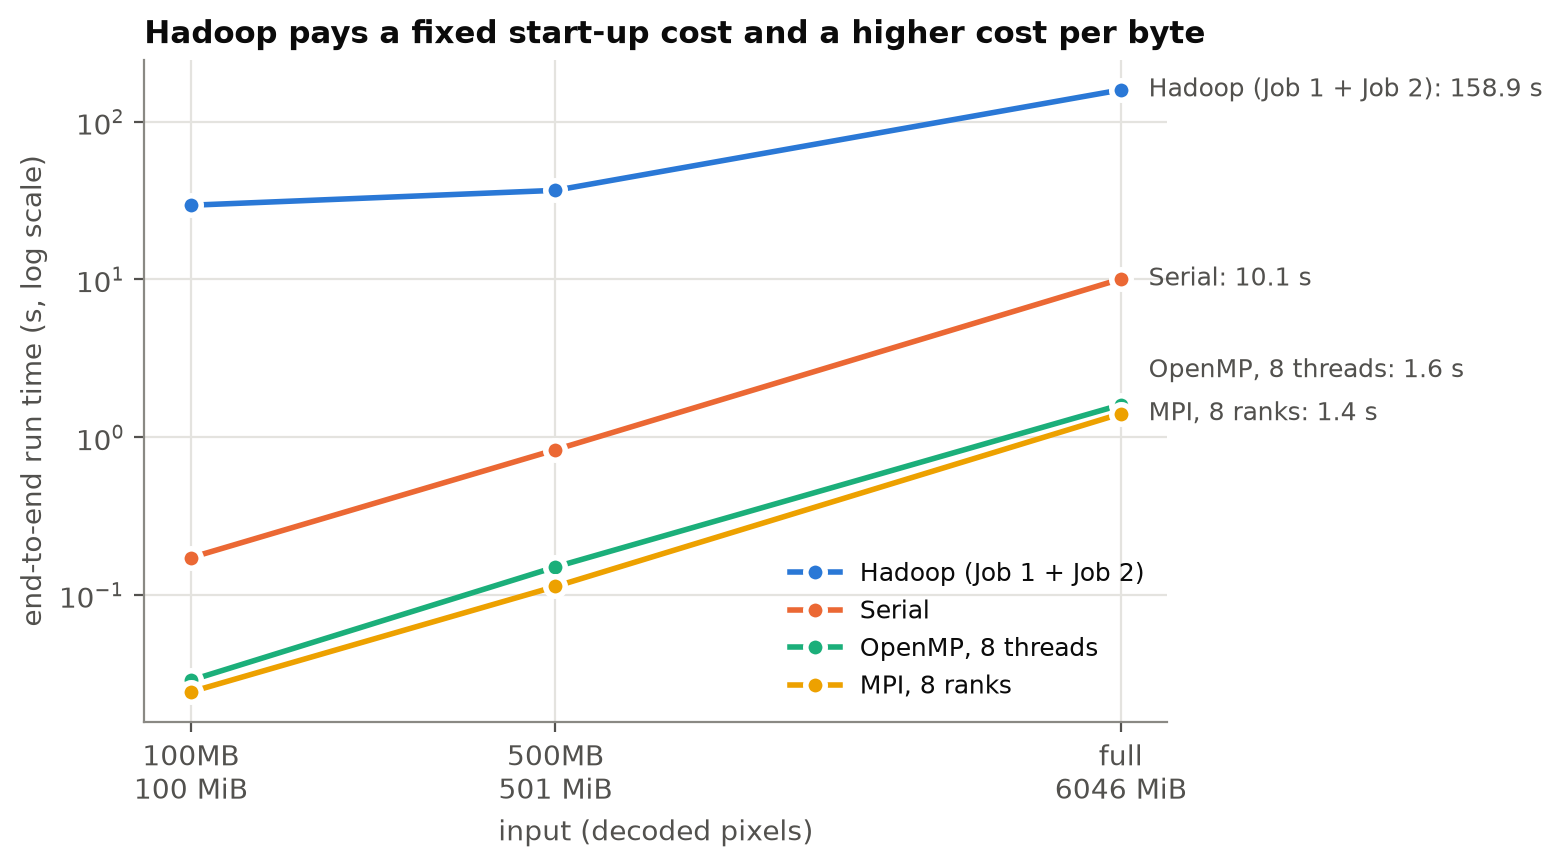
\includegraphics[width=\linewidth]{../plots/phase3/compare.png}\caption{}\end{subfigure}\hfill
\begin{subfigure}{0.46\linewidth}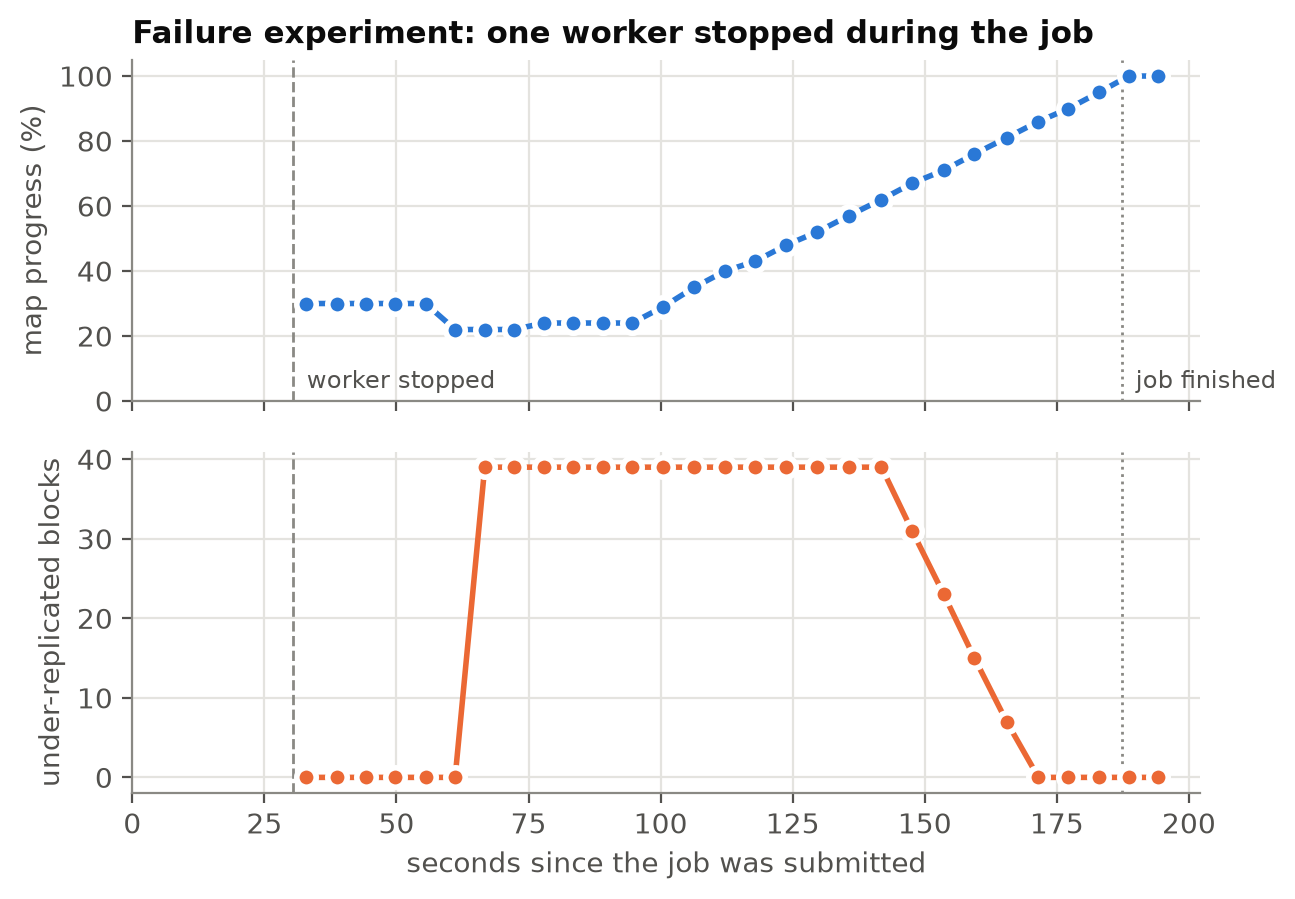
\includegraphics[width=\linewidth]{../plots/phase3/failure.png}\caption{}\end{subfigure}
\caption{(a) Run time against input size for the four models. (b) The failure experiment.}
\label{fig:p3}
\end{figure}

\emph{Why Hadoop is slower on small inputs.} A line through the 100MB and full runs gives a
\textbf{fixed cost of about 27\,s per pipeline}: two client JVMs, two ApplicationMasters, a JVM
per task container, and scheduling driven by one-second heartbeats. The 100MB set itself needs
0.17\,s of computation, so the run is almost entirely start-up. \emph{Where it would win.} On
this cluster, never: Hadoop's marginal cost is 21.8\,ms per MiB against 1.66\,ms for the serial
program. It spent 135\,s of CPU on the full set, 13 times the serial program, decoding base64,
moving megabyte-long lines through the JVM and the streaming pipes, and reading the input
twice. With ideal scaling it would need about 13 busy cores to match the serial program and
about 96 to match 8 MPI ranks. Hadoop therefore pays off not on speed at this scale but when
the data no longer fits one machine, or when the job is long enough that a node failure is
likely, because it is the only model here that survives one.

\paragraph{Combiner experiment.} We ran Job 1 with and without \texttt{-combiner} and compared
the job counters (Table~\ref{tab:combiner}).

\begin{table}[H]
\centering\small\setlength{\tabcolsep}{4.5pt}
\begin{tabular}{llrrrrrr}
\toprule
Set & Combiner & Map out & Comb. in & Comb. out & Reduce in & Shuffle bytes & Time (s) \\
\midrule
500MB & yes & 2{,}988 & 2{,}988 & 627 & 627 & 23{,}699 & 18.9 \\
500MB & no & 2{,}988 & 0 & 0 & 2{,}988 & 101{,}046 & 17.7 \\
full & yes & 35{,}958 & 35{,}958 & 966 & 966 & 38{,}810 & 81.0 \\
full & no & 35{,}958 & 0 & 0 & 35{,}958 & 1{,}215{,}993 & 79.2 \\
\bottomrule
\end{tabular}
\caption{Job 1 counters with and without \texttt{-combiner} (records; medians).}
\label{tab:combiner}
\end{table}

The mapper emits six records per training image. Without a combiner all 35{,}958 cross the
network to the reducer. With it, each map task first adds up its own records per key, so only
966 leave the 63 map tasks: \textbf{31 times less shuffle traffic} (1{,}188\,KiB down to
38\,KiB). The result is unchanged because integer addition is associative and commutative. The
job is not faster (81.0 against 79.2\,s): our shuffle is tiny next to the map work, and the
combiner adds a process per map task. A combiner pays off when the map output is large relative
to the map computation, which is not our case.

\paragraph{Failure experiment.} We started Job 1 on the full set and, at 27\,\% map progress,
stopped one worker: its NodeManager and its DataNode (Figure~\ref{fig:p3}b).

\begin{table}[H]
\centering\small
\begin{tabular}{lrrrr}
\toprule
\texttt{hdfs fsck} & DataNodes & Under-replicated & Avg. replication & Status \\
\midrule
before & 3 & 0 & 2.00 & healthy \\
36\,s after the stop & 2 & 39 of 63 blocks & 1.38 & healthy \\
141\,s after the stop & 2 & 0 & 2.00 & healthy \\
after the worker rejoined & 3 & 0 & 2.00 & healthy \\
\bottomrule
\end{tabular}
\caption{HDFS during the failure experiment. ``Healthy'' means no block has lost all replicas.}
\end{table}

\textbf{The job finished and its result is still bit-exact.} It launched 69 map attempts
instead of 63: 6 were killed and rerun, and none counted as failed, because attempts lost with
a node do not count against a task's retry limit. It took 187\,s instead of 81\,s. The
NameNode re-created the 39 missing replicas on the two remaining DataNodes on its own, and
\texttt{yarn node -list} showed the node as \texttt{LOST}.

This is the \emph{partial failure} of the first lecture: one component died while the rest kept
running, and the rest could not know it had died. For about 35\,s nothing happened
(Figure~\ref{fig:p3}b), because a dead node and a slow node look identical until a heartbeat
timeout expires; we had shortened those timeouts from Hadoop's default of about 10 minutes to
20--30\,s. Then map progress went \emph{backwards}, from 30\,\% to 22\,\%: map outputs are
stored on the worker's local disk, not in HDFS, so the completed maps of the lost node had to
be redone as well. Recovery is re-execution, which is only correct because the tasks are
deterministic and their outputs are committed atomically. We deliberately spared the node
running the ApplicationMaster; losing it restarts the whole job attempt.

\paragraph{Consistency and replication.} HDFS keeps all metadata in one NameNode, so namespace
operations are strongly consistent. Files are write-once with a single writer (a lease), and a
block is written through a pipeline to all its replicas before it is acknowledged, so the
replicas of a closed block are identical and a reader may use any of them. A replica that
missed updates while its node was down carries an old generation stamp and is discarded when
the node returns (when our worker rejoined, its replicas were surplus and replication stayed at 2.00); corrupted replicas
are caught by checksums and read from another copy. Our pipeline needs little more: its input is
immutable, each task attempt writes to its own temporary directory and is committed by an atomic
rename, so although tasks run \emph{at least once}, each output appears \emph{exactly once}.
Stronger guarantees would cost availability and latency. Synchronous replication already makes
writes slower with every replica; requiring all replicas to be reachable would block writes
whenever a DataNode is down (with replication 1 we saw the opposite trade: less space, no
safety); allowing several writers or in-place updates would need locking or consensus per block;
and the single NameNode that makes metadata consistent is also a single point of failure.

%======================================================================
\section{Bonus work}
%======================================================================

\begin{itemize}
  \item \textbf{Hybrid MPI + OpenMP.} \texttt{build/mpi -t N} runs OpenMP inside each rank.
    $1\times8$, $2\times4$, $4\times2$ and $8\times1$ give the same compute time within 2\,\%.
  \item \textbf{CUDA} (\texttt{src/cuda/}). Resize, per-image sums and normalization run on the
    GPU in batches of 256 images, bit-exact. The kernels need \textbf{0.11\,s for the whole
    set}, but the run takes 3.69\,s (2.7$\times$ over serial, slower than 8-core OpenMP at
    1.36\,s): staging 0.92\,s, upload 0.87\,s, download 1.35\,s and host-side CRC 0.48\,s.
    Moving the pixels to the card and 8.3\,GiB of results back over PCIe costs about 27 times
    more than computing them.
  \item \textbf{RPC query service} (\texttt{src/rpc/}). A TCP server answers \texttt{STATS},
    \texttt{CLASS k} and \texttt{IMAGE id} from the MapReduce output; the client has a timeout
    and retries. With a 500\,ms timeout, a server that replies after 2\,s and one that never
    replies produce the same client output. A client cannot distinguish slow from crashed: both
    are ``no reply yet''. Retrying is safe only because our requests are idempotent reads.
  \item \textbf{Second MapReduce job}: Job 2 above, and per-class statistics in Job 1.
\end{itemize}

%======================================================================
\section{Reflection}
%======================================================================

\paragraph{Limitations of MapReduce} that we met in practice:
\begin{enumerate}
  \item \textbf{High fixed latency.} About 13\,s per job before any record is processed makes
    it unusable for small or interactive work (171 times slower than serial on 100\,MB).
  \item \textbf{No state between stages.} Our computation needs one global result between its
    two passes. In MapReduce that is two jobs, and the second re-reads and re-decodes the whole
    input from disk. Iterative algorithms pay this in every iteration.
  \item \textbf{Record-oriented text I/O.} Binary images must become base64 lines: 33\,\% more
    bytes and 13 times the CPU time.
  \item \textbf{Intermediate data is not replicated.} Losing a node loses its finished map
    outputs, so completed work is repeated.
\end{enumerate}

\paragraph{Limitations of our study.} Both clusters are containers on one laptop: the network
is a virtual bridge and all nodes share one memory system, disk and clock limit. The dataset is
5.9\,GiB, far below the scale Hadoop is built for. Hadoop's detection timeouts were shortened.
GPU timings include a consumer laptop's PCIe link.

\paragraph{Lessons learned.}
\begin{itemize}
  \item \textbf{Make the result exact, then verify everything.} An integer specification let six
    implementations in five programming models be checked bit for bit, in every experiment,
    including the one where a node was killed.
  \item \textbf{Measure before explaining.} Three of our expectations were wrong: that dynamic
    scheduling would win, that a first cache benchmark measured memory (the compiler had removed
    the loop), and that a GPU would be fastest end to end.
  \item \textbf{Move the computation to the data.} The MPI design that reads locally scales
    perfectly; every design that funnels data through one place (a collector rank, a PCIe link,
    a single reducer) is limited by that place.
  \item \textbf{Each model buys something different.} OpenMP: the least code. MPI: the best
    end-to-end time. Hadoop: 16 to 171 times slower here, and the only one that finished
    correctly after losing a machine.
\end{itemize}

\end{document}
